\section{Data Access}

The initial phase of FedCampus operates on participants' health data recorded by
the Huawei Watch Fit 2.
100 smartwatches of this model are purchased to be lent to the participants.

As a ground truth, to preserve user privacy,
the bottom line is that the raw data must not be collected.
However, in order to conduct research on the data,
our algorithms need to access the data from the smartwatch.

To deploy algorithms without collecting raw data,
we need to deploy the algorithms on users' edge devices and
access the data there.
In the natural life cycle of the collected health data,
the data are first synchronized from the participants' smartwatches to
the Huawei Health Kit~\cite{huaweihealthkit} on
their smartphone through Bluetooth.
This is important in two ways:
first, we do not need to develop any software to run on the smartwatches,
only the smartphones; second,
we require the participants to regularly conduct this synchronization process
themselves, which counts into management complexity.

We deploy different strategies to access the data from the Huawei Health Kit on
Android and iOS.
On Android, Huawei provides the Huawei Health Kit API to access the data.
On iOS, Apple restricts third-party access to private data,
and unifies such access to Apple HealthKit~\cite{applehealthkit},
so we have to first synchronize the data from the Huawei Health Kit to
the Apple HealthKit, then access the data via Apple HealthKit.

\section{The \fedcampus Application}

The major challenge of the \fedcampus Application is to
support both Android and iOS devices.
This is necessary because our participants at Duke Kunshan University are
a mix of Android and iOS users,
and we want to allow as many of them to participate as possible.
However, Android and iOS applications are incompatible,
and developing separate applications for these two platforms would be
a laborious task because
it would mean we have to maintain two separate codebases and
duplicate any changes.

To support mobile development on both Android and iOS,
we leverage the Flutter application framework.
Instead of developing two separate applications for Android and iOS,
by using Flutter,
only a single codebase is needed to for both the Android and iOS versions of
the application.
Therefore, we implement as much of the \fedcampus Application on Flutter as
possible to maximize our code reuse and minimize our development effort.

\section{Designing \fedkit}

As an overview, \fedkit is a software development kit designed to
facilitate federated learning among clients running on Android and iOS devices.
Since smartphone operating systems vendors generally lock down their
operating systems to only access external software as "applications",
our clients in this case are the smartphone application.
To orchestrate and control the federated learning process,
we also need a backend server to schedule training on the clients and
manage machine learning model aggregation.

\subsection{Challenges in \fedkit's Design}

The design of \fedkit faces three major challenges:

\begin{enumerate}
\item To leverage the potential participant pool at Duke Kunshan University,
    the \fedcampus Application needs to support both Android and iOS devices.
    This means that any federated learning system we integrate into it
    also needs to support both Android and iOS devices.
    However, existing on-device training frameworks for smartphones typically
    only support either of these two platforms,
    which means that we have to implement every machine learning models twice
    and train them separately on Android and iOS,
    splitting our participants' data and
    losing part of the point of federated learning.
\item Typical machine learning examples on smartphones from major frameworks
    include the machine learning models inside the applications themselves,
    which couples updating the models with updating the applications.
    However, application updates possibly need to go through a review process
    in the vendor's application store, or require users intervention.
    These processes take the control out of the hands of the \fedcampus team,
    and pose difficulties in iterating the machine learning model in production.
\item Integrating any federating learning process into
    the \fedcampus Application requires both mobile development knowledge
    for the implementation,
    and machine learning knowledge for the actual algorithm.
    These intertwined requirements means that the software developer and
    the data scientist on the \fedcampus team have to work very closely for
    any federated-learning-related features and adjustments,
    resulting in high development overhead.
\end{enumerate}

To address the first challenge,
we design a cross-platform federated learning model pipeline to
support the whole federated learning process,
from model creation, deployment, training, to aggregation,
which we present in Section~\ref{sec:pipeline}.
For the second challenge,
our federated learning workflow enables flexible machine learning operations
from the backend in production,
as we detail in Sec.~\ref{sec:mlops}.
The entire procedure tackles the third challenge by
providing a user-friendly development environment in Python for
all the tasks related to machine learning model creation and
algorithm deployment.

% TODO: Paraphrase the content of this subsection.
\subsection{Cross-Platform Federated Learning Model Pipeline}
\label{sec:pipeline}

To enable cross-platform federated learning,
especially \textit{cross-platform aggregation},
we propose a pipeline comprising
\textit{model conversion} and
\textit{unified training APIs},
as shown in Fig.~\ref{fig:pipeline}.

\begin{figure}\begin{center}
    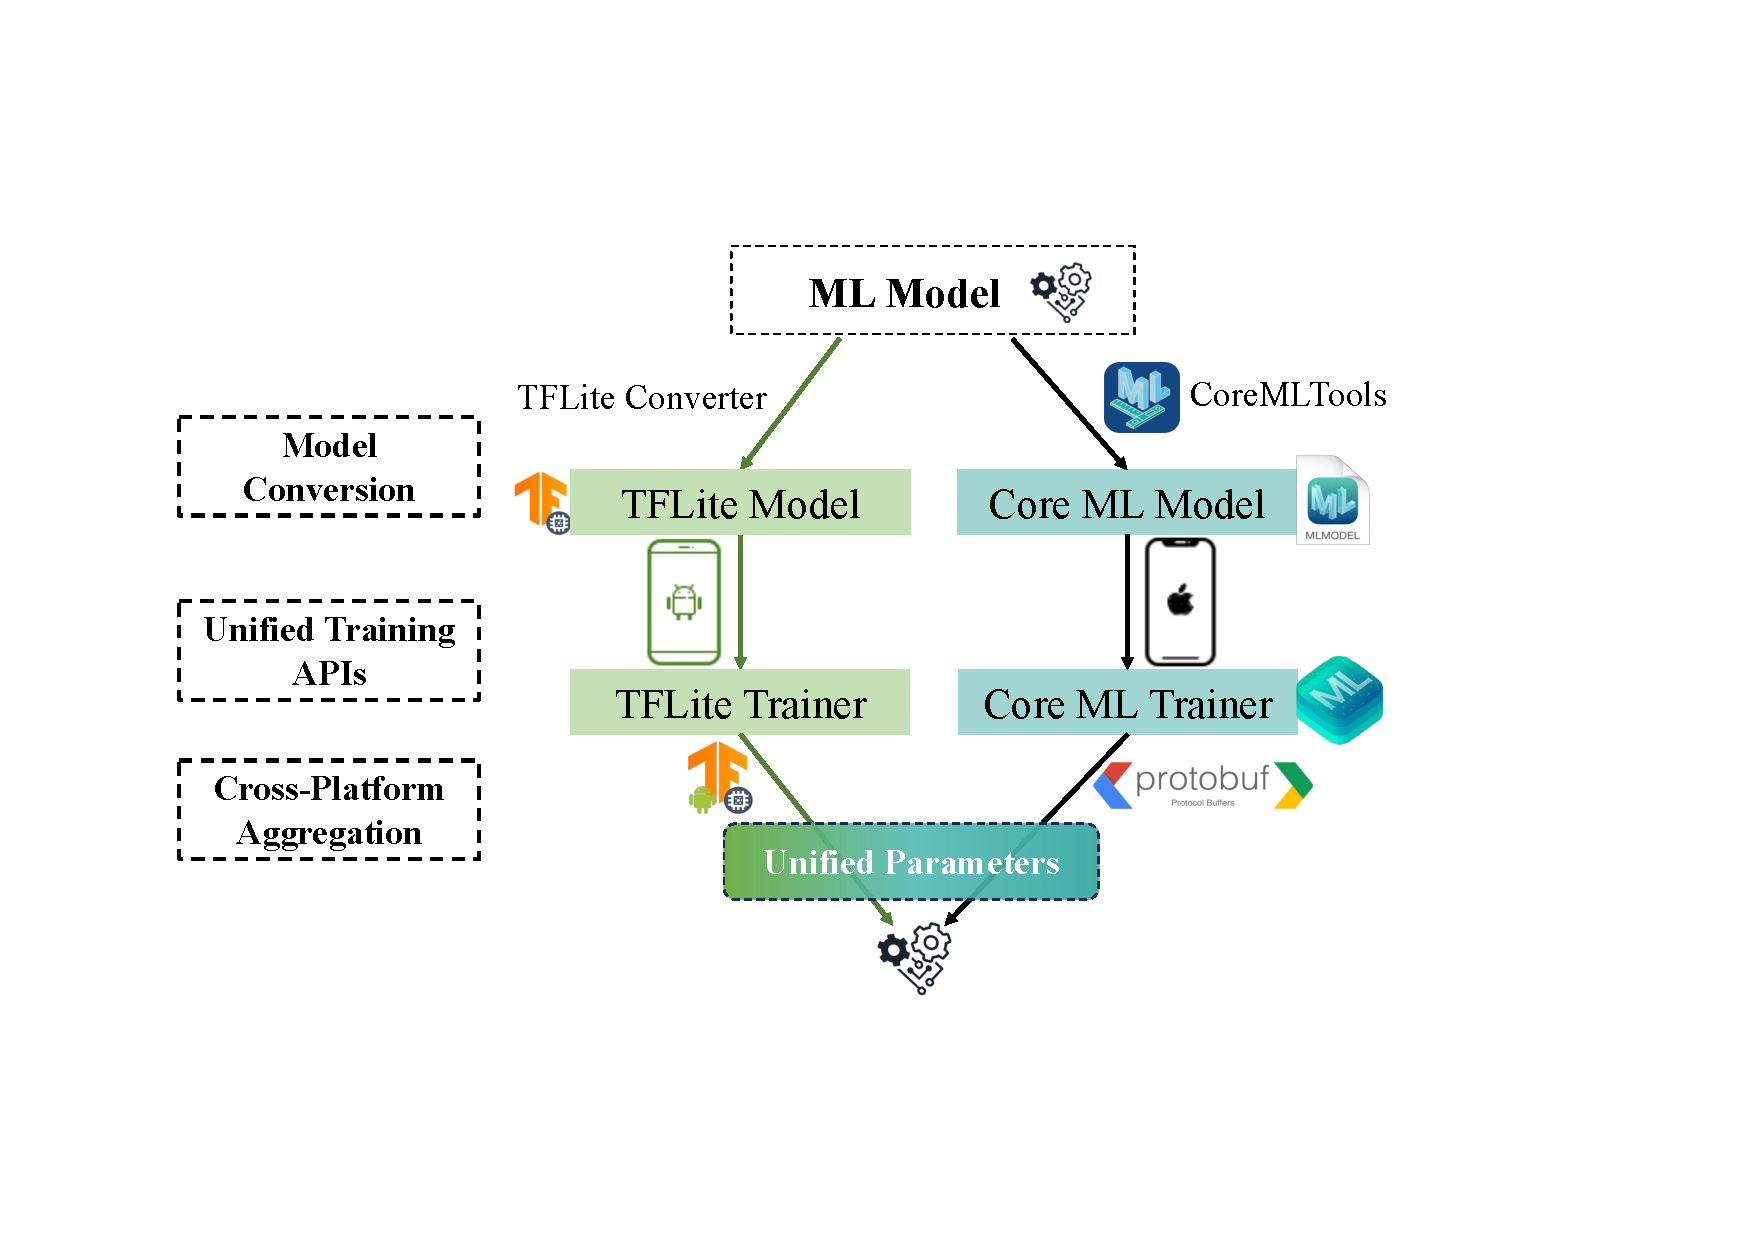
\includegraphics[width=\linewidth]{model_pipeline.pdf}
    \caption{\fedkit Model Pipeline for Cross-Platform Federated Learning.}
    \label{fig:pipeline}
\end{center}\end{figure}

\subsubsection{Model Conversion}
To enable model creation in Python,
we begin by converting models into formats compatible with
Android (TensorFlow Lite or TFLite) and iOS (Core ML).
Core ML defines a fixed model structure and provides
the official converter CoreMLTools.
For TFLite, we standardized a model format, and then
developed a compliant TensorFlow converter.
This standardized format includes
four essential federated learning methods
(\textsf{train}, \textsf{infer}, \textsf{parameters},
and \textsf{restore}).

\subsubsection{Unified Training APIs}
\fedkit provides \textit{TFLite Trainer} and \textit{Core ML Trainer} to
train the converted models on Android and iOS devices,
utilizing GPU and NPU acceleration.
Moreover, both trainers expose unified APIs for
\textit{retrieving and setting model parameters,
    model fitting, and evaluation}.
On Android, these APIs invoke the TFLite interpreter to call
our \textit{standardized methods} defined in \textit{Model Conversion}.
However, on iOS, our experimentation revealed that
Core ML \textit{forbids} directly setting parameters, which could impede federated learning.
To overcome this constraint,
we modify the underlying ProtoBuf representations of
Core ML models.
Specifically,
we employ Swift code generated from the relevant ProtoBuf definition files,
and navigate nested model definitions to access parameters on iOS.
Consequently, our unified training APIs exhibit comparable functionality on
both iOS and Android platforms.

\subsubsection{Cross-Platform Aggregation}
Aggregation necessitates
\textit{uniform parameter representations},
which poses primary challenges in
retrieving and setting parameters for Core ML and TFLite.
1)~Core ML permits \textit{only} specific layers to be \textit{updatable} and
only provides their parameters post-training.
Thus, to obtain \textit{other layers'} parameters,
we implemented a solution using ProtoBuf manipulation.
This approach involves recording layer information
during \textit{Model Conversion} and
utilizing it during training.
2)~The TFLite interpreter only accepts inputs/outputs as maps from
\textit{names} to \textit{tensors}.
Therefore, during \textit{Model Conversion},
we assign index-based names to each parameter layer and
dynamically generate the concrete methods that accept these arguments.
During training, we call the methods with these index-based names to
access parameters.
Finally, these unified parameters enable seamless cross-platform aggregation.

% TODO: Fit this in.
\subsubsection{On-Device Training}

The FedScale benchmark~\cite{lai2022fedscale} takes an interesting approach to
run TensorFlow on Android---it uses the Termux Application to
create a UNIX shell environment.

% TODO: Paraphrase the content of this subsection.
\subsection{Machine Learning Operations}
\label{sec:mlops}

\newcommand{\model}{$M$}
\newcommand{\fs}{$S_\mathrm F$}
In production,
federated learning development faces challenges from
the lack of direct control over end devices.
\fedkit empowers researchers to deploy models and algorithms continuously (MLOps).
Leveraging our complete control of the self-hosted Backend,
\fedkit's three-step federated learning workflow
facilitates continuous delivery and training,
as illustrated in Fig.~\ref{fig:fl-workflow}.

\begin{figure}\begin{center}
    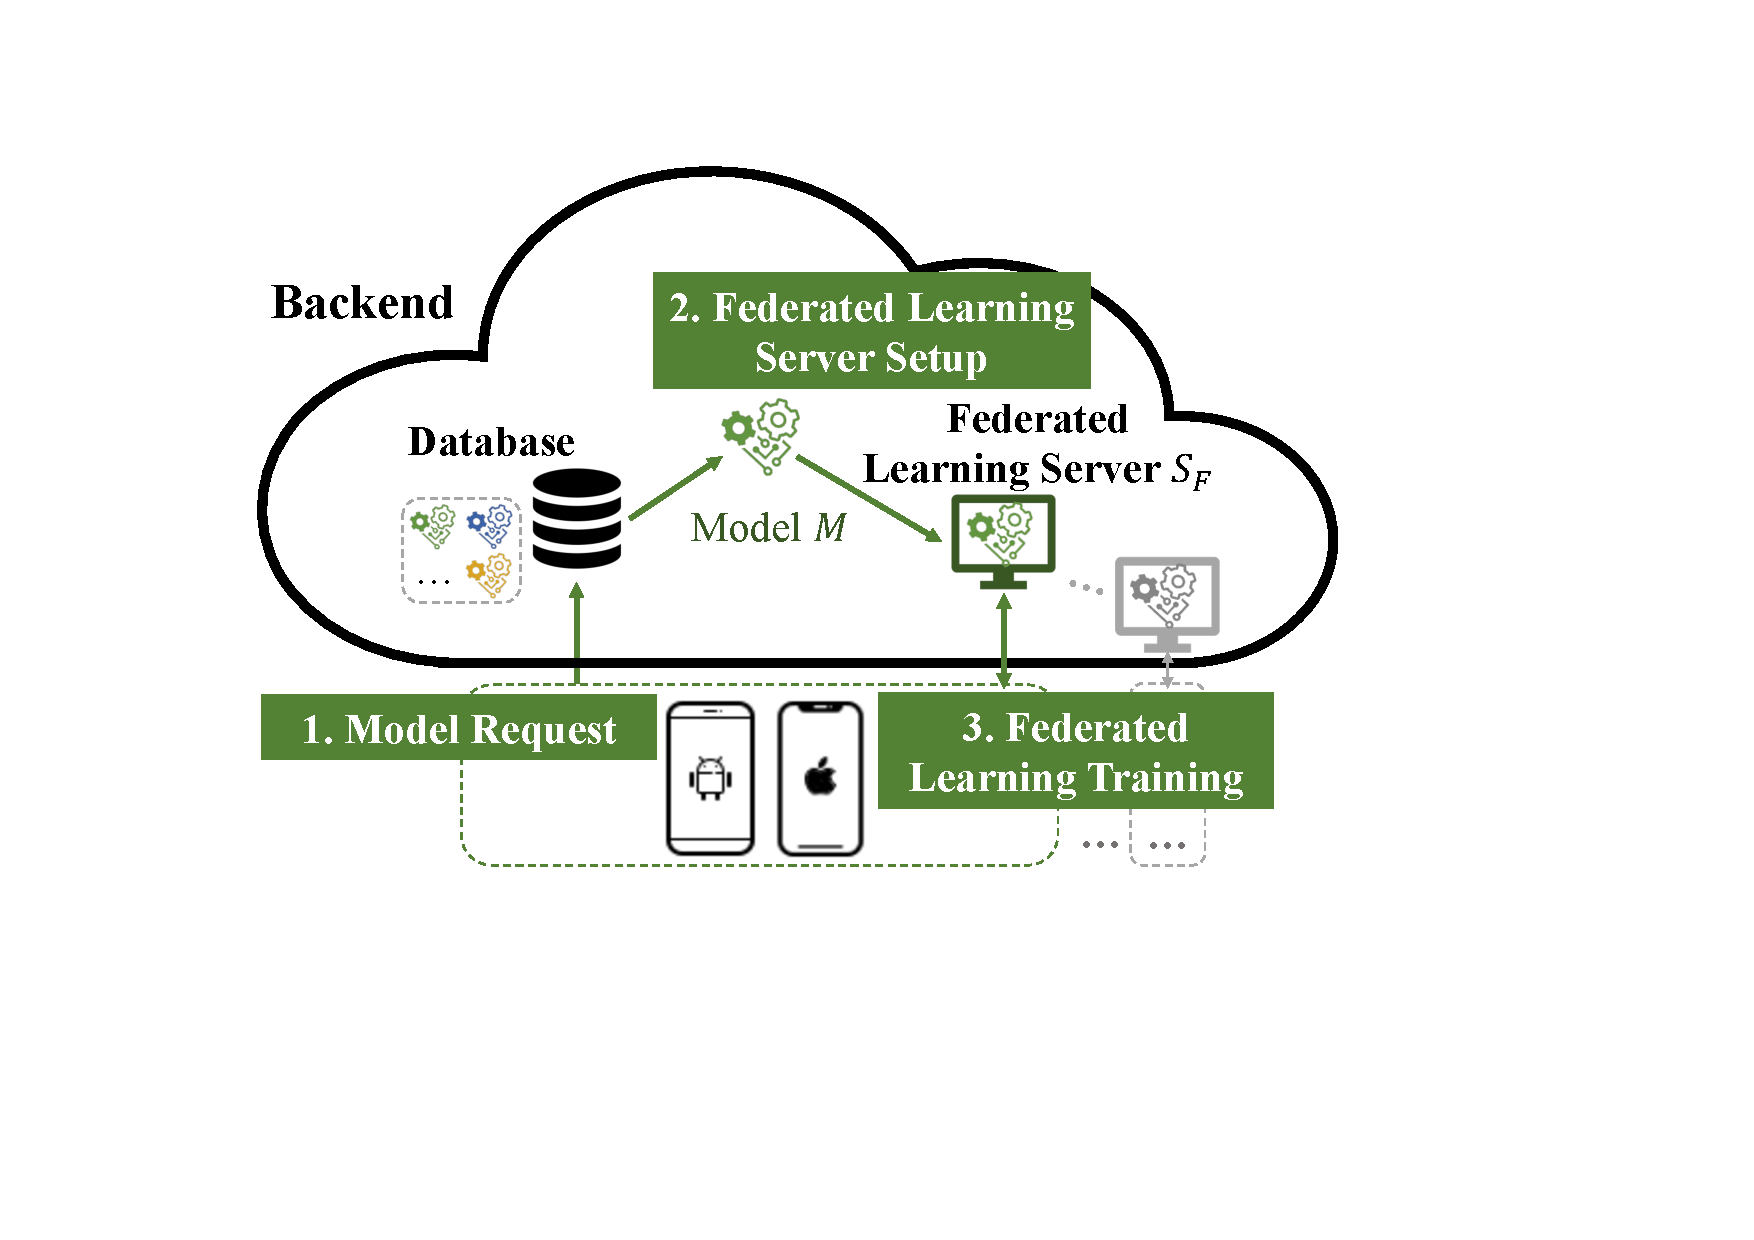
\includegraphics[width=0.7\linewidth]{fl_workflow.pdf}
    \caption{\fedkit federated learning Workflow.}
    \label{fig:fl-workflow}
\end{center}\end{figure}

\subsubsection{Continuous Cross-Platform Model Delivery}
Traditionally, models for on-device training are \textit{embedded} into client apps.
However, this approach couples model delivery with app updates,
resulting in complexities when submitting apps to app stores and garnering user adoption.

Circumventing this complexity,
\fedkit enables \textit{continuous model delivery without app updates} by
decoupling models from clients through \textit{Model Request},
which allows new model deployment by uploading to the Backend.
Specifically, clients request the Backend for a model (TFLite/Core ML)
aligned with
their platform (Android/iOS) and training data type.
The Backend selects the appropriate model \model{} from the database and
responds with detailed model information.
Consequently, \textit{Model Request} delivers the TFLite or Core ML model
to clients for federated learning training.

\subsubsection{Customizable Continuous federated learning Training}
\fedkit manages continuous federated learning training by allowing \textit{multiple parallel federated learning training sessions}
through federated learning server Setup.
When clients request an federated learning server to
train their chosen model \model{},
the Backend either reuses a suitable federated learning Server \fs{} if it exists,
or spawns a new one.
Each federated learning server
operates as an independent Python subprocess of the Django Backend,
occupying its own port that
clients connect to for federated learning Training.
This dynamic approach ensures that
newly delivered models can be immediately trained with new federated learning servers
without affecting ongoing ones.
Furthermore,
these federated learning servers employ the Flower federated learning Framework for
scheduling training and evaluation.
This decision empowers our federated learning servers to leverage Flower's flexibility and
allow for federated learning algorithm customizations in Python.
